\documentclass[12pt]{article}

\usepackage{units}
\usepackage[colorlinks=true]{hyperref}
\usepackage{graphicx}
\usepackage{mathtools}
\usepackage{amsmath}

\DeclareMathOperator{\arctanh}{arctanh}

\newcommand{\Teff}{\mathrm{T_{eff}}}
\newcommand{\twTeff}{\mathrm{\tilde{T}_{eff}}}

\begin{document}

\title{\texttt{GDit}: a Python library for gravity darkening corrections to stellar evolution models}
\author{Aaron Dotter}

\maketitle

\begin{abstract}
Rotating stars are subject to gravity darkening, in which the flux
at the stellar surface is not uniformly distributed. As a consequence
a rotating star appears both hotter and brighter at the poles than
at the equator. This document describes a method to derive surface-averaged
gravity darkening corrections that can be applied to stellar evolution models.
These adjust the intrinsic model effective temperature, surface gravity, and
luminosity in order to account for the effects of gravity darkening as well as
the orientation of the observer relative to the stellar rotation axis. I introduce
\texttt{GDit}, a Python module to calculate these corrections as well as a
simple means of applying them to stellar evolution models. The code and this document
are available from the \href{https://github.com/aarondotter/GDit}{Github repo}.
\end{abstract}


\section{The gravity darkening model}
The gravity darkening model is derived by Espinosa Lara \& Rieutord (2011,
A\&A, 533, 43; hereafter ELR). ELR assume the radiative flux is directed
antiparallel to the effective surface gravity. The effective surface gravity
is not uniform in a rotating star and, thus, neither is the flux. Since the
scalar flux (F) is related to the effective temperature ($\Teff$) by the
Stefan-Boltzmann law, the same
argument applies to both F and $\Teff$. The ELR model reduces to a differential
equation characterized by two variables: the polar angle $\theta$ and the ratio
of surface angular velocity to the Keplerian angular velocity (ELR eq.\ 10):
\begin{equation}
  \omega = \frac{\Omega}{\Omega_K} = \Omega \sqrt{ \frac{R_e}{GM} }
\end{equation}
where $\Omega$ is the surface angular velocity (radians per second,
assumed uniform), $\Omega_K$ is the Keplerian angular velocity,
$R_e$ is the equatorial radius of the star, $G$ is Newton's gravitational constant,
and $M$ is stellar mass. 

The ELR model is valid for $0 \leq \theta \leq \pi/2$; all other values of
$\theta$ are mapped into this interval via symmetry arguments. The model
requires a numerical solution, except at the extrema $\theta = 0$ (ELR eq.\ 27)
and $\pi/2$ (ELR eq.\ 28) for which analytical solutions are provided. The
numerical solution boils down to finding the value of $\tilde{r}=R/R_e$ that
satisfies (ELR eq.\ 30)
\begin{equation}
  \frac{1}{\omega^2 \tilde{r}} + \frac{1}{2} \tilde{r}^2 \sin^2 \theta = \frac{1}{\omega^2} + \frac{1}{2}
\end{equation}
for given $\omega$ and $\theta$. The values of $\tilde{r}$, $\theta$, and $\omega$ are then used to solve for the modified angular variable $\vartheta$ (ELR eq.\ 24)
\begin{equation}
  \cos \vartheta + \ln \tan(\vartheta/2) = \frac{1}{3} \omega^2 \tilde{r}^3 \cos^3 \theta + \cos \theta + \ln \tan(\theta/2)
\end{equation}
These are straightforward to solve with a root-find and, at this point one can calculate the normalized temperature variable
\begin{math}
  \twTeff = \Teff \left( \frac{L}{4 \pi \sigma R_e^2} \right)^{-1/4}
\end{math} via ELR eq.\ 31.

\begin{figure}
  \centering
  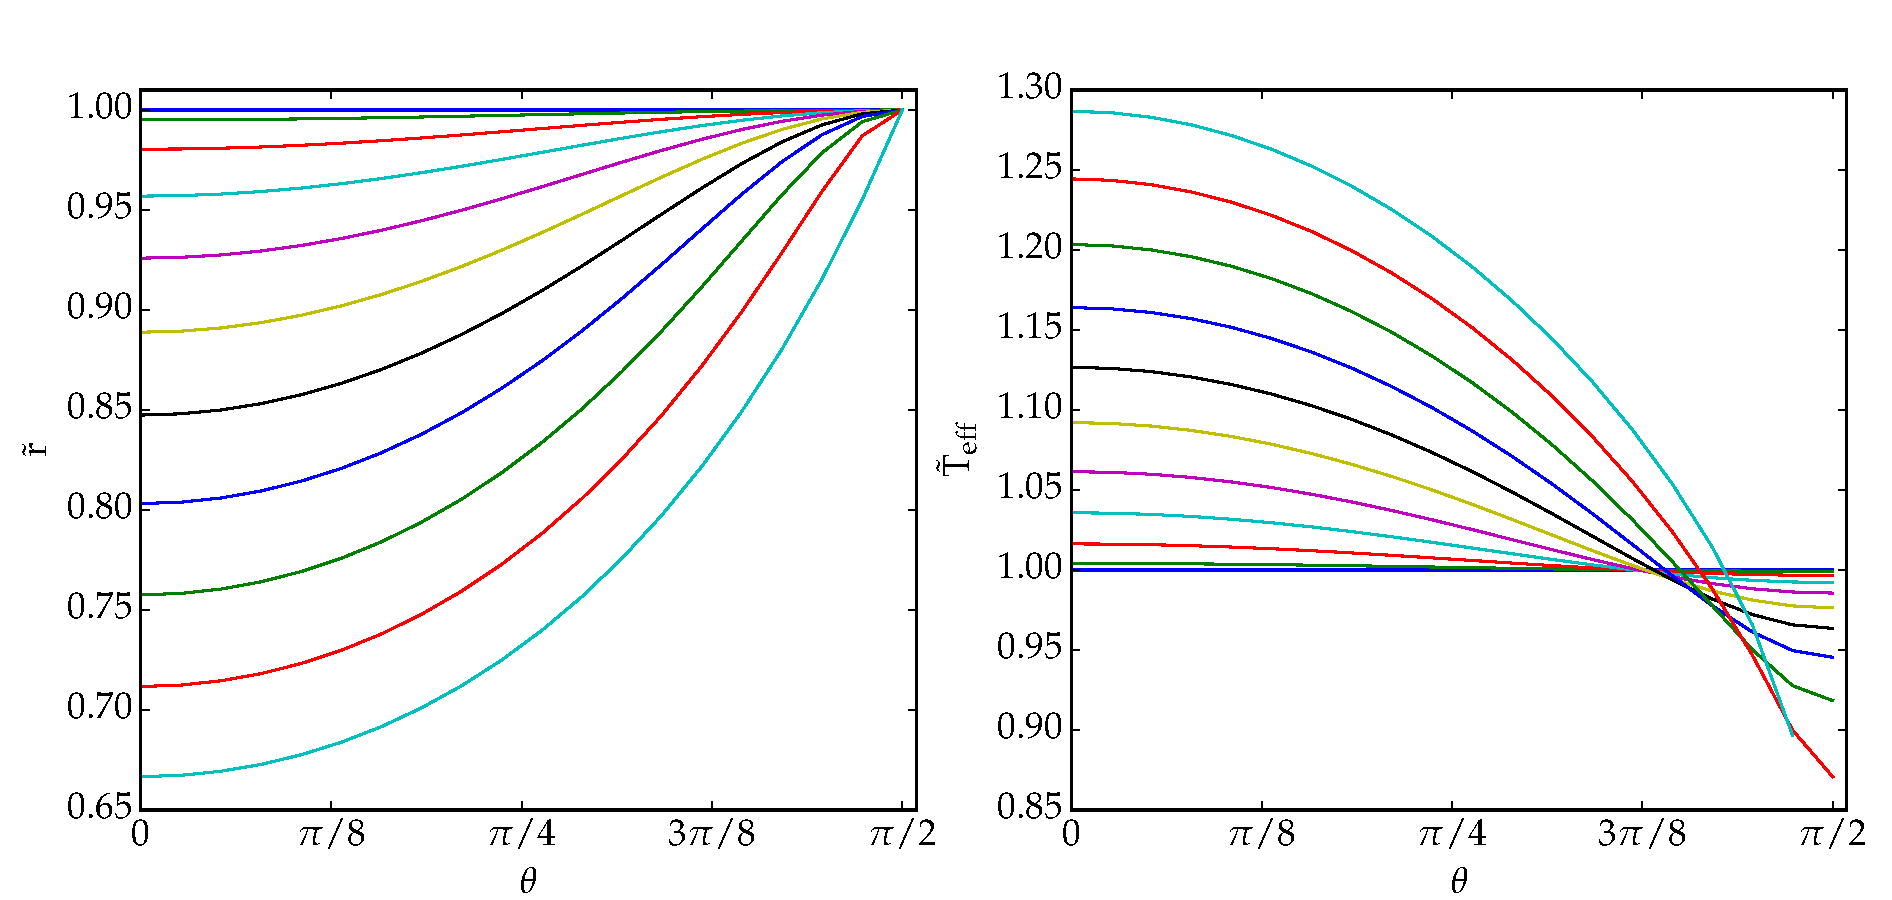
\includegraphics[width=0.99\textwidth]{../plots/R_and_T.pdf}
  \caption{Solution of the ELR model for $0 \leq \omega \leq 1$; each curve is a different value of $\omega$. \emph{Left:} The ratio of the stellar radius to the equatorial radius ($\tilde{r}=R/R_e$) as a function of the polar angle $\theta$ for different values of $\omega$. \emph{Right:} Similar to the left panel but now showing $\twTeff$, see text for details. Recall that $\theta=0$ corresponds to the pole and $\theta=\pi/2$ to the equator.\label{fig:ELR}}
\end{figure}

Figure \ref{fig:ELR} shows the solution of the ELR model as a function of
$\theta$ for different values of $\omega$. Figure \ref{fig:ELR} indicates
that the polar radius reaches a minimum value of $R_p = (2/3) R_e$ at $\omega=1$.
$\twTeff$ is included in the right panel of Figure \ref{fig:ELR}. When
$\omega=0$, the idealized star is spherical and, thus, $R_p = R_e$ and
$\twTeff = \Teff$ for all $\theta$. When $\omega=1$, $\twTeff$ varies by as much
as $\sim25\%$ between the pole and the equator.

\section{Oblateness and projection effects}
Now that we have a solution for the ELR model we can begin to
compute the projected luminosity along the line of sight (LOS). The surface is
an oblate spheroid so we work in oblate spheroidal coordinates. The coordinate
system is defined by three variables: polar angle $\nu$, azimuthal angle
$\phi$, and $\mu$ = $\arctanh( R_p /R_e )$. It is important to distinguish
between $\nu$ in the oblate spheroidal coordinate system and the polar angle
$\theta$ in the ELR model: $\nu = 0$ at the equator; $\nu = \pi/2$ at the pole
and, thus, $\theta = \pi/2 - \nu$. Note also that, due to azimuthal symmetry
in this problem, there is no explicit $\phi$-dependence in the following.

With the oblate spheroidal coordinate system thus defined, and properly
connected to the ELR model, we can now integrate over the stellar surface
($\Sigma$). However, the quantity that we want is that projected along the line
of sight (LOS) and for that we need to define one additional angle, $i$, and the
LOS unit vector $\hat{l}(i)$. $i$ is chosen such that $i = 0$ at the equator.
The projected surface is denoted $\Sigma_{proj}$.

An analytical formula to calculate $\Sigma_{proj}$ (the area of an ellipse) for
arbitrary orientation of an ellipsoid is given by Binggeli~(1980, A\&A, 82, 289; eqs.\ 2 \& 3).
The area of an ellipse is $\pi~a~b$ and we take $a=R_e$. Then the problem reduces
to finding the ratio of the semi-minor axis to the semi-major axis ($\beta = b/a$)
of the projected ellipse, which simplifies, for an oblate spheroid, to
\begin{equation}
\beta = \sqrt{ \frac{j + 1 - \sqrt{ (j-1)^2}}{j+1+\sqrt{(j-1)^2}} }
\end{equation}
where, using $q=R_p/R_e$ and $\alpha=\pi/2-i$, 
\begin{equation}
j = q^2 \sin^2 \alpha + \cos^2 \alpha
\end{equation}
Finally, the projected area is 
\begin{equation}
  \Sigma_{proj} = \pi \beta R_e^2
\end{equation}
Note that Brandt \& Huang (2015, ApJ, 807, 58) use a different formula that is only
correct at $i = 0$ and $i=\pi/2$. Compared to Binggeli's formula, the
Brandt \& Huang formula leads to a maximum error of $\sim8\%$ in $\Sigma_{proj}$
at $i = \pi/4$.

To calculate the luminosity projected along the LOS, $L_{proj}$, requires the
surface integral
\begin{equation}\label{eq:lproj}
  L_{proj} = 4 \iint \limits_{d\vec{\Sigma} \cdot \hat{l} > 0} F d\vec{\Sigma} \cdot \hat{l}
\end{equation}
where only the flux projected toward the observer,
i.e., $d\vec{\Sigma} \cdot \hat{l} \geq 0$, is kept.
Once $L_{proj}$ and $\Sigma_{proj}$ are known, the projected effective temperature,
$\Teff_{,proj}$, can be obtained from the Stefan-Boltzmann law
\begin{equation}
\Teff_{,proj} = \left( \frac{L_{proj}}{\sigma \Sigma_{proj}} \right)^{1/4}
\end{equation}
where $\sigma$ is the Stefan-Boltzmann constant.

\begin{figure}
  \centering
  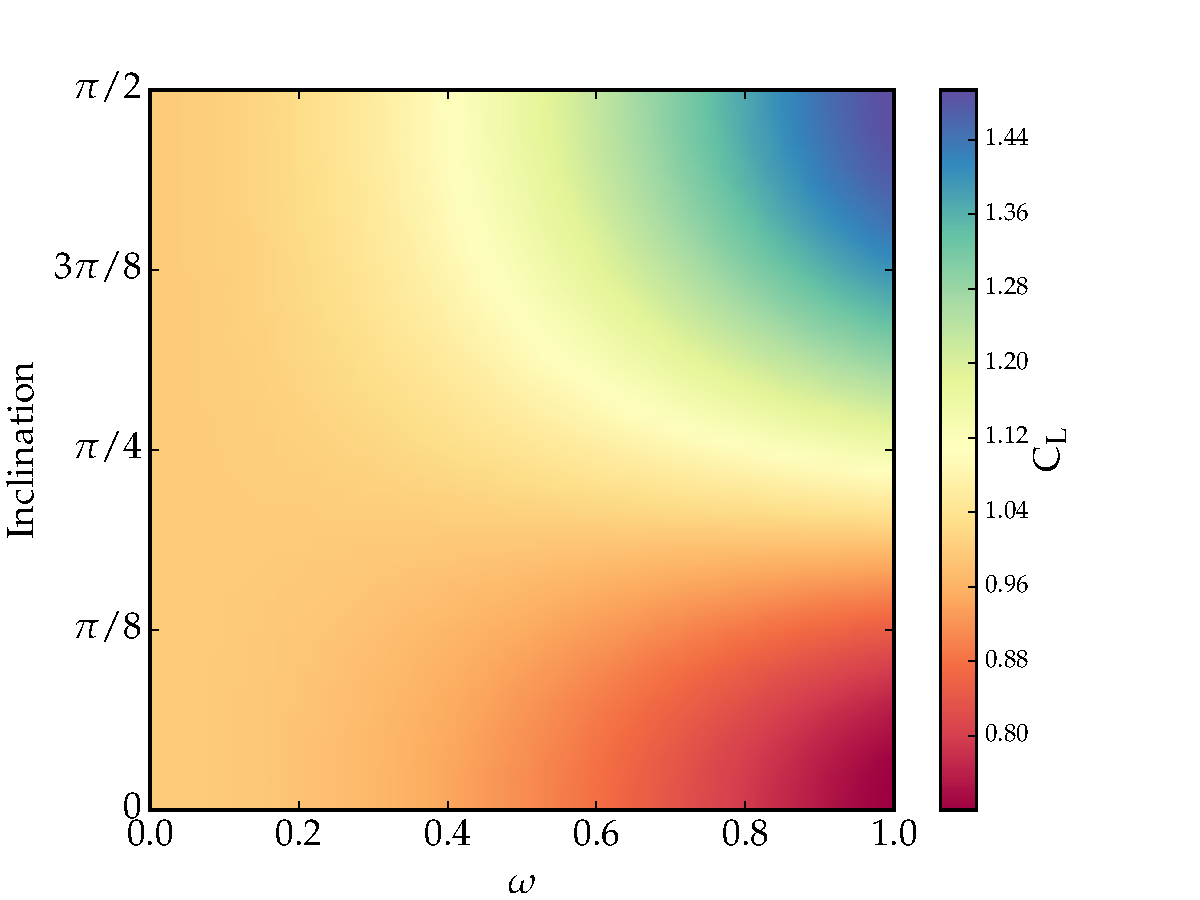
\includegraphics[width=0.9\textwidth]{../plots/C_L.pdf}
  
  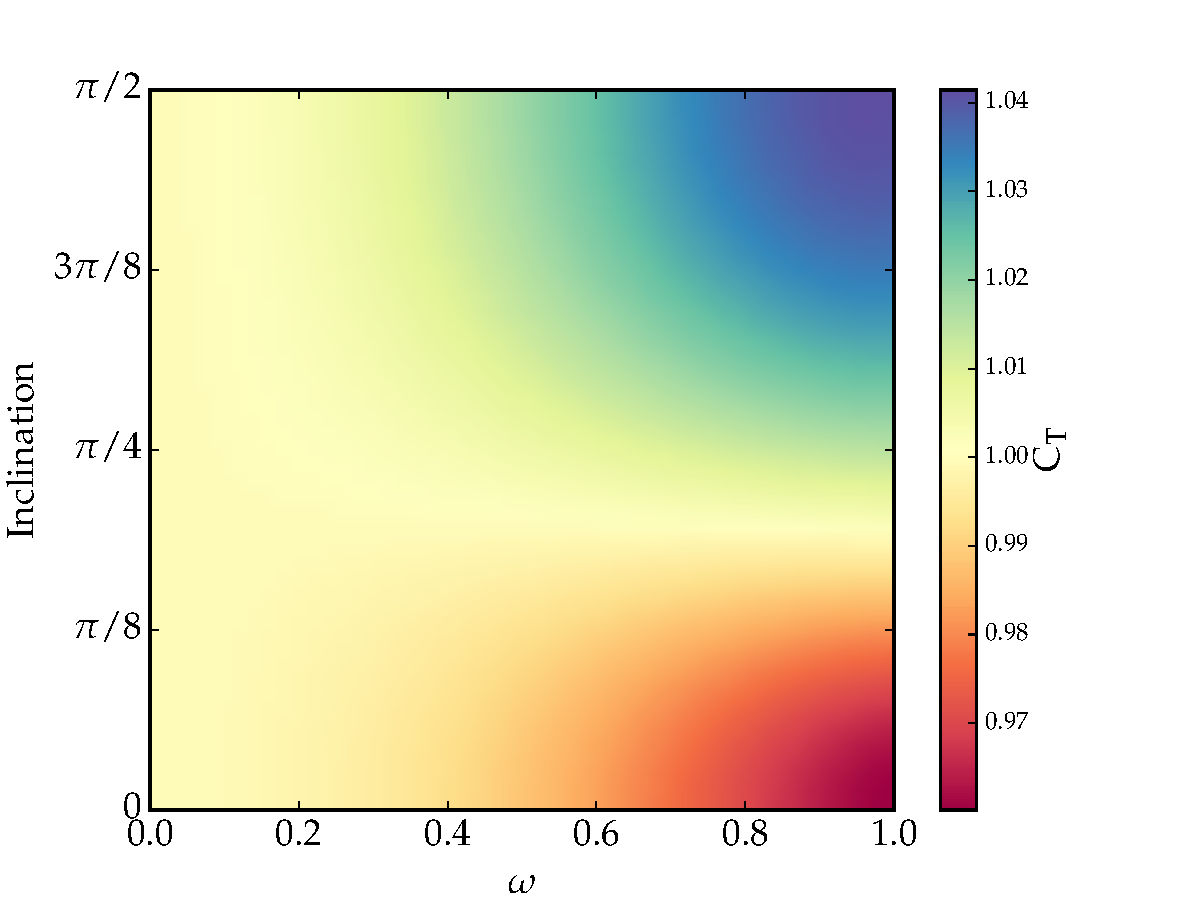
\includegraphics[width=0.9\textwidth]{../plots/C_T.pdf}
  
  \caption{The range of $C_L$ (upper panel) and $C_T$ (lower panel). Note the
    color scale is different in the two panels. \label{fig:coeff}}
\end{figure}


The following is based closely on what is done in the SYCLIST code
(Georgy et al.\ 2014, A\&A, 566, 21). The double integral (\ref{eq:lproj}) is a
geometric factor that does not depend on the stellar temperature or luminosity.
It only depends on $\omega$ and $i$. Thus, it makes sense to derive correction
factors which allow the projected quantities to be determined from the model
intrinsic quantities by geometric scaling factors, i.e.,
\begin{equation}
  L_{proj}(\omega,i) = C_L(\omega,i) L
\end{equation}
and
\begin{equation}
  \Teff_{,proj}(\omega,i) = C_T(\omega,i) \Teff
\end{equation}
Thus defined, the geometric factors $C_L$ and $C_T$ are given by
\begin{equation}
C_L = \frac{L_{proj} }{\iint\limits_\Sigma F d\Sigma}
\end{equation}
and
\begin{equation}
C_T = \left( \frac{C_L \Sigma}{4 \Sigma_{proj}} \right)^{1/4}
\end{equation}

Figure \ref{fig:coeff} shows how the values of $C_T$ and $C_L$ vary over the
$\omega$,$i$-plane. These can be compared with the upper panels of Figure 2
in Georgy et al.\ (2014). The variation of $C_L$ is greater than that of $C_T$
due to the $\nicefrac{1}{4}$-power relationship between the two. At $\omega=1$, where
the geometric factors are the largest, $C_L$ varies from $-25\%$ to
$+50\%$ while $C_T$ varies by $\pm4\%$. When the LOS is oriented at
$i=34^{\circ}$ ($0.6$ rad) above the equatorial plane, both $C_L~,~C_T \simeq 1$
for all $\omega$.

\section{Python code for $C_T$ and $C_L$}
The github repository provides Python code to numerically solve the differential equations in the ELR model
and to compute the geometric coefficients $C_L$ and $C_T$ for arbitrary $\omega$ and $i$. The repository
also includes a Python interface to interpolate $C_L$ and $C_T$ coefficients from a $50\times50$ grid
stored in a data file.  Separate interpolants are provided for $C_L$ and $C_T$ to enable the application
of gravity darkening corrections to stellar evolution models. As an example, Figure \ref{fig:HRD} shows
a MIST isochrone (Choi et al.\ 2016, ApJ, 823, 102) with $\omega=0.4$ (at the ZAMS). The left panel shows
the intrinsic $\Teff$ and luminosity as well as the gravity-darkened values for $i=0$ and $i=90^{\circ}$.
The right panel shows how $\omega$ evolves along the isochrone from the initial value of $\omega=0.4$ set
at the ZAMS. The most dramatic differences in the H-R diagram occur when $\omega$ is large. $\omega$ is
provided in MIST as \texttt{surf\_avg\_omega\_div\_omega\_crit}.

\begin{figure}
  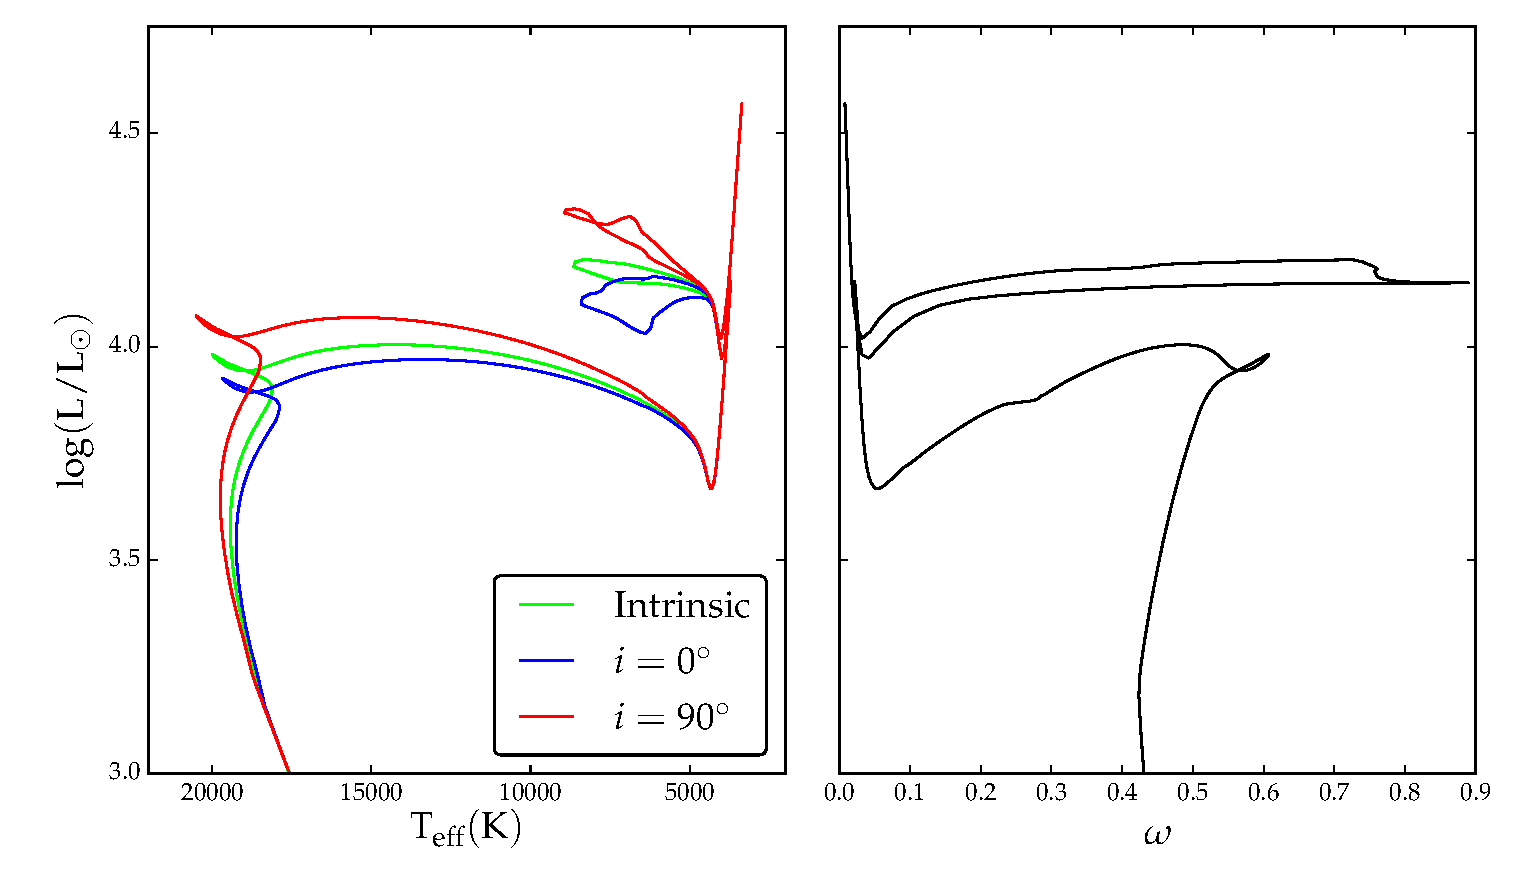
\includegraphics[width=0.9\textwidth]{../plots/iso.pdf}
  \caption{MIST isochrone with [Fe/H]=0, log(age[yr])=7.5, and $\omega=0.4$ at the ZAMS.
    \emph{Left:} The H-R diagram showing the effect of changing the inclination angle $i$ from
    $0^{\circ}$ (in the plane of equator) to $90^{\circ}$ (aligned with the rotation axis). \emph{Right:}
    The variation in $\omega$ with luminosity to explain why the gravity darkening correction
    is larger or smaller at a given point on the isochrone in the H-R diagram. \label{fig:HRD}}
\end{figure}

\end{document}
